\documentclass[PI,LAB]{HSEUniversity}
% Возможные опции: KR или VKR; PI или BI
\usepackage{svg}
\usepackage{listings}

\title{Оценка архитектуры программной системы для заданной предметной области}
\author{Виноградов Никита Андреевич}
\supervisor{к.т.н., доцент кафедры Информационных технологий в бизнесе НИУ ВШЭ-Пермь}{А.В.~Кычкин}

\Year{2020}


% Ссылка на файл с описание библиографии
\bibliography{library.bib}

%%%%%%%%%%%%%%%%%%%%%%%%%%%%%%%%
%%% ТЕКСТ РАБОТЫ %%%%%%%%%%%%%%%
\begin{document}

% Обязательные элементы оформления: заголовочный слайд, аннотация, оглавление
\maketitle



\chapter{Оценка архитектуры программной системы для заданной предметной области. }
\section {Описание проекта}
\emph{Описание проекта} - Автоматизированная система нагрузочного тестирования для веб-серверов (облачных систем).

\emph{Цель проекта} - Автоматизировать и упростить процесс тестирования нагрузки и последующего исследования показателей для принятия решений.

\emph{Задачи проекта} -

\emph{Области применения} - Облачные  распределенныые системы,  ETL и MapReduce системы.

\emph{Составные части}:
\begin{enumerate}
	\item Сервер системы - выполняет роль единой точки обращения к системе, позволяет назначать работы для воркеров и управленяет работой Воркеров.
	\item Воркеры - рабочие элементы системы выполняющие роль тестировщиков, в данной системе  они могут выполнять 2 вида работ:
	      \begin{enumerate}
		      \item Hit-Based тестирование.
		      \item Сценарное тестирование.
	      \end{enumerate}
	\item Мониторинг - используется для просмотра информации о проведенных нагрузочных тестах, составлении графиков зависимостей.
	\item Сборщик логов - используется для сбора информации со всех элементов системы и записи процесса выполнения на диск, для последующей отладки или просмотра.
	\item Агенты - помощники основной системы, в основной части выполняются на target машине для которой выполняется тестирование чтобы отследить данные по процессору, памяти, дисковой нагрузке, также агенты  используется для предотвращения падения системы в случае высокой нагрузки сервера нагрузочного тестирования.
	\item Планировщик - используется для организации работ, которые выполняют воркеры.В текущей системе распределяет потоки выполнения для увеличения общей вычислительной мощности.
	\item Веб-Сервер - используется для загрузки конфигурации нагрузочных тестов и просмотра информации по возможностям системы и свободным воркерам.
	\item CLI-клиент - клиент системы выполняющий функции веб-сервера, только в режиме терминала.
\end{enumerate}






\section {Компоненты системы}
\begin{enumerate}
	\item Генератор запросов - используется самописный генератор Http/Https запросов на Golang и C++ со вставки на NASM, данное решение было принято после тестирования существующих генераторов и определения узких мест.
	\item СУБД - для данной системы была выбрана колоночная Time-Series База данных ClickHouse. Данное решение обусловлено  возможностями системы по предоставлению нагрузки и генерации метрик в ходе тестирования, (Было проведено  тестирование возможностей системы и при режиме тестирования \emph{максимальной производительности}, система может выдавать 1.8 Млн RPS) в ходе этого необходимо эффективно доставлять метрики в базу данных а не копить в памяти сервера.
	\item Jenkins X Api Client - инструмент для подключения к  системе сборки и доставки приложений.
	\item  Gitlab CI/CD  Api Client - инструмент для подключения к  системе сборки и доставки приложений.
	\item Kubernetes Api Client - инструмент для подключения к системе оркестрации контейнеров, будет использовать для проверки масштабирования компонентов облачных систем.
	\item Webhooks -инструменты создания конечных точек в системе на сервере, для выполнения определенных команд.
	\item gRPC - инструмент эффективного подключения сервисов внутри и между дата-центрами с помощью подключаемой поддержки для балансировки нагрузки, трассировки, проверки работоспособности и аутентификации
	\item TabiX - инструмент для анализа данных из ClickHouse и построения графиков и диаграмм по тестируемым системам
\end{enumerate}


\section {Архитектурный стиль}


\begin{FIGURE}[h]{Диаграмма компонентов системы системы{\tiny}\label{fig:example-figure}}
	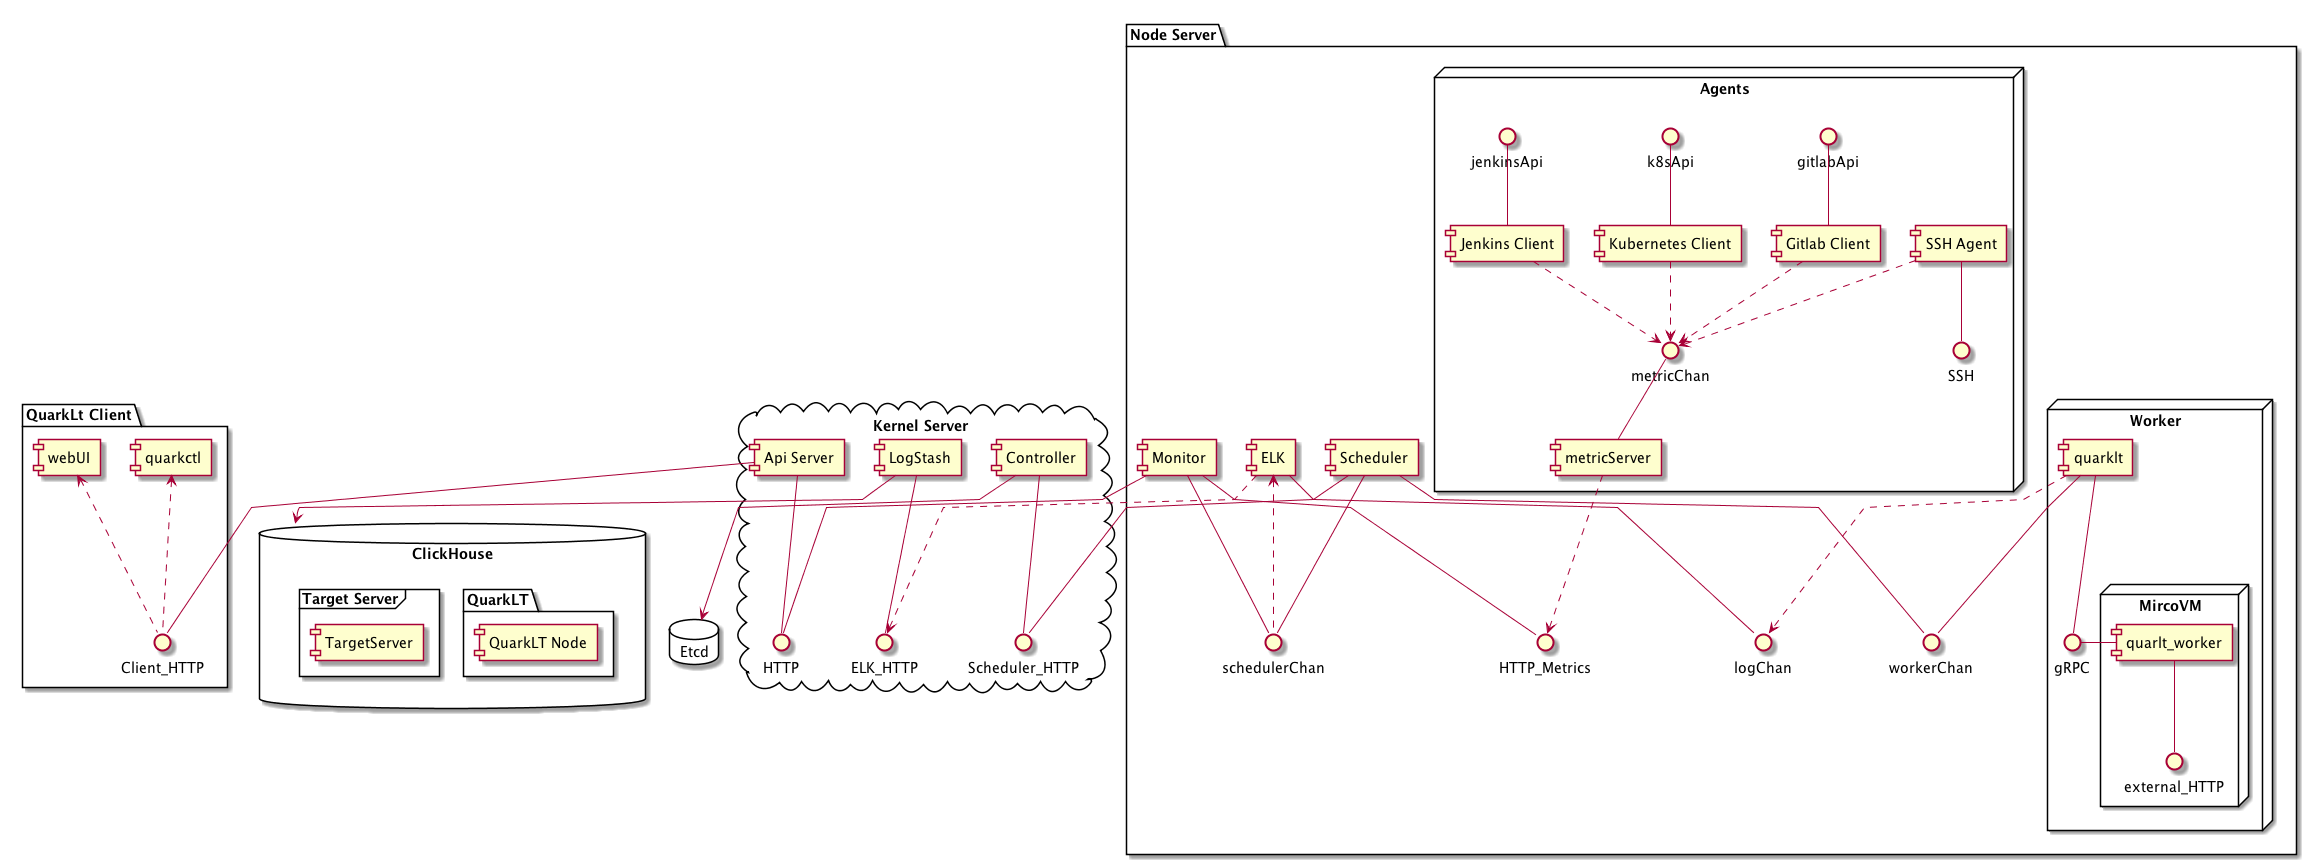
\includegraphics[angle=90,width=0.5\textwidth]{out/diag/component/component}
\end{FIGURE}
\begin{enumerate}
	\item Клиент-Сервер - используется для взязи CLI CLient и Воркеров в сервером системы.
	\item Master-Slave - используется для масштабирования воркеров, в задачах тестирования серверов с большими возможностями.
	\item Observer - используется для сбора логов и метрик в компонентах системы.
\end{enumerate}







\chapter{Диаграмма вариантов использования проектируемой системы в соответствии с нотацией UML}

\begin{FIGURE}[h]{Диаграмма прецедентов системы{\tiny}\label{fig:example-figure}}
	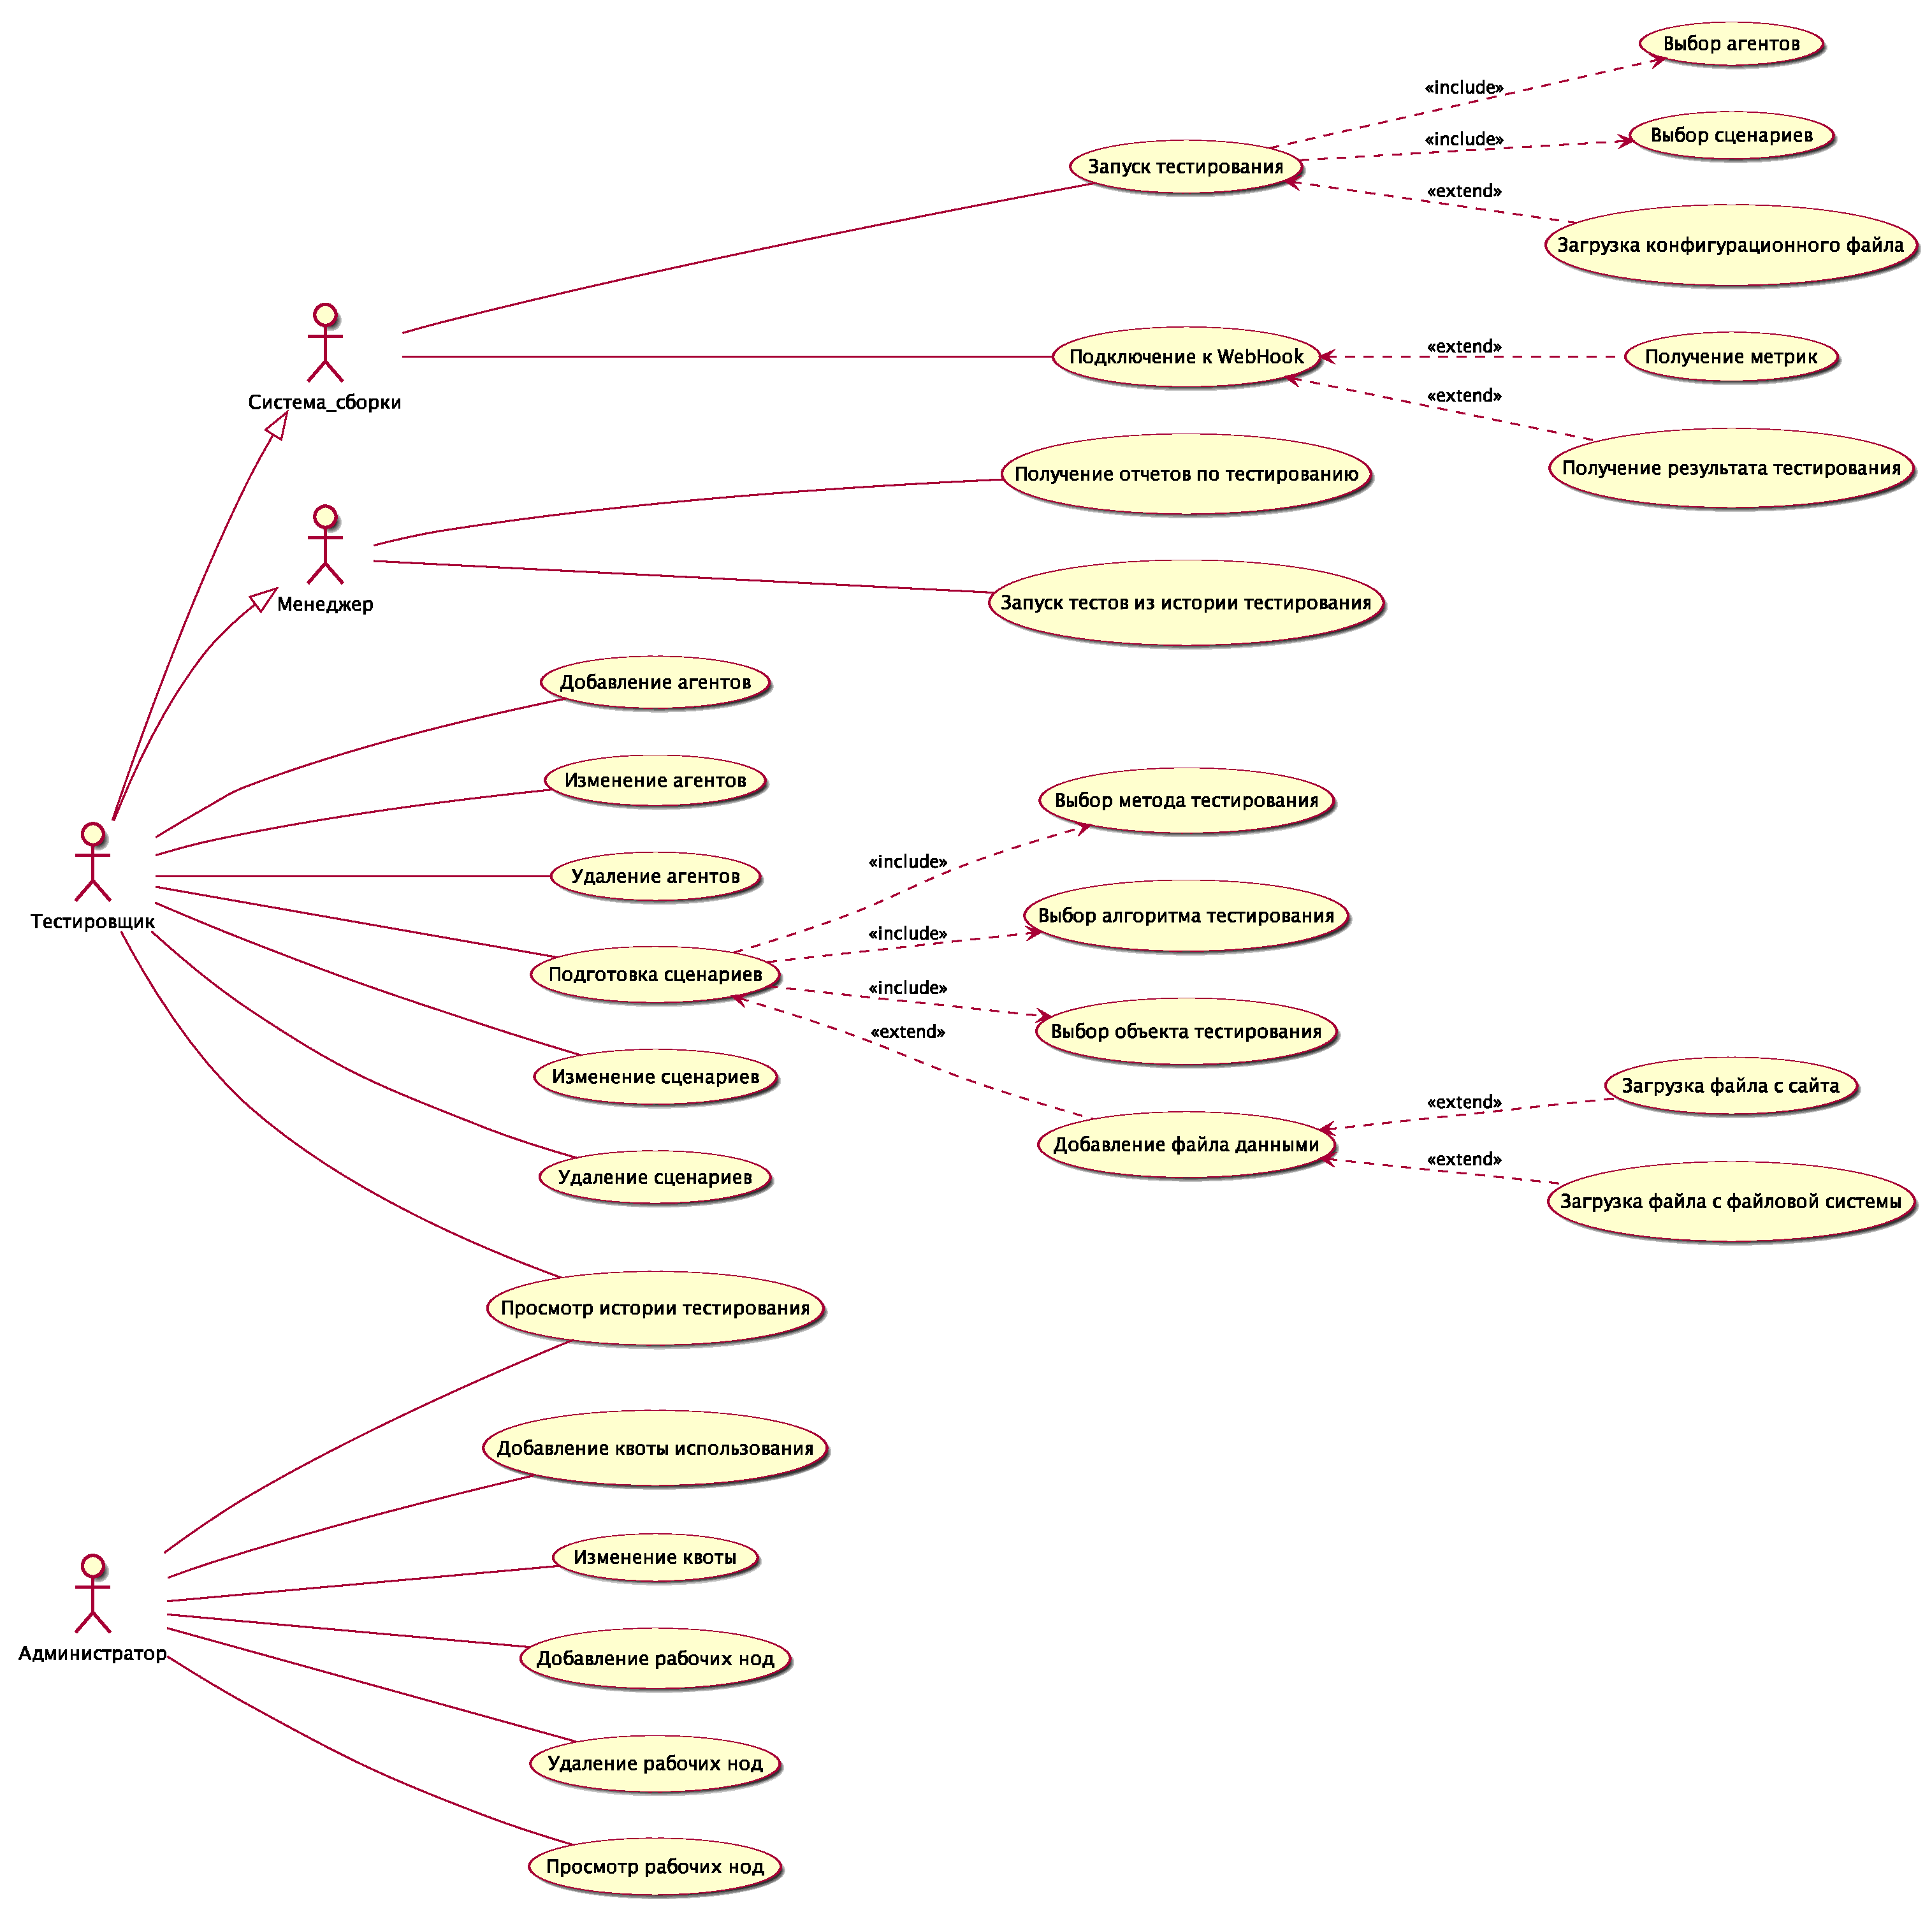
\includegraphics[width=1\textwidth]{out/diag/use-case/use-case}
\end{FIGURE}

\chapter{Архитектура информационной системы для заданной предметной области с использованием выбранного архитектурного решения}



\section{Диаграммы активности и последовательности}
Диаграммы активносности и последовательности описаны ниже \newline
\textbf{Наименование}: Добавление рабочих нод.\newline
\textbf{Обязанности}: Добавить рабочие ноды\newline
\textbf{Ссылки}:  прецедент «Добавление рабочих нод». \newline
\textbf{Предусловия}: Администратор зашел в систему и выбрал <<Добавление рабочих нод>>.\newline


\begin{FIGURE}[h]{Диаграмма последовательности {\tiny}\label{fig:example-figure}}
	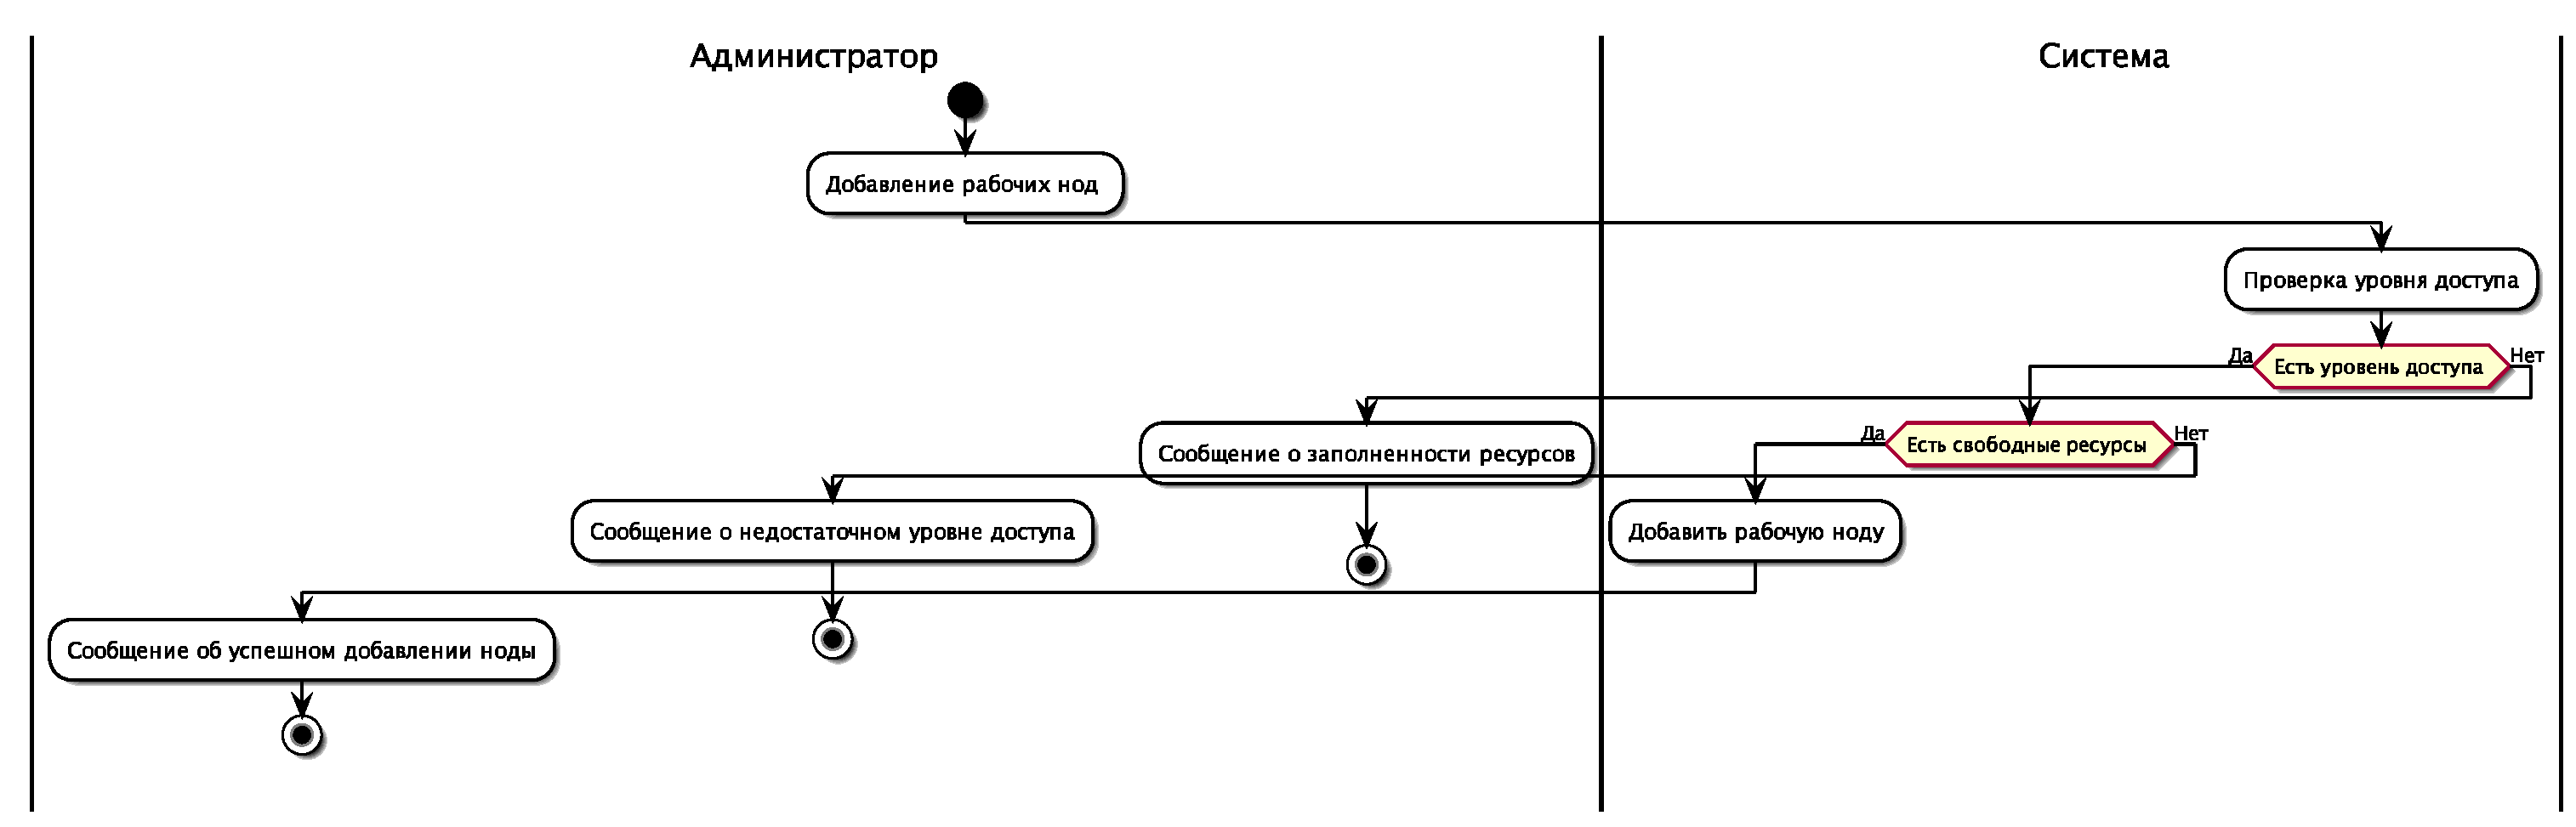
\includegraphics[width=1\textwidth]{out/diag/add_worker_node/add_worker_node}
\end{FIGURE}

\end{document}
